\documentclass[10pt]{article}
\usepackage[utf8]{inputenc}
\usepackage{listings}
\usepackage{float}
\usepackage{graphicx}
\usepackage{fullpage}
\usepackage{caption}
\usepackage{subcaption}
\usepackage{amsmath}
\usepackage{hyperref}

%\renewcommand{\thesubsection}{\arabic{subsection}}
\renewcommand{\thesubsubsection}{\alph{subsubsection}}

\title{Pattern Recognition Practical 5}
\author{Group 24: \and Maikel Withagen (s1867733) \and Steven Bosch (s1861948)}
\date{\today}
\lstset{
frame=single, 
numbers=left, 
breaklines=true, 
language=Matlab,
basicstyle=\footnotesize, 
title=\lstname,
showstringspaces=false
}

\renewcommand{\thesection}{Assignment \arabic{section}}
\renewcommand{\thesubsection}{\arabic{subsection}}
\begin{document}
\maketitle

\section{k-means clustering, quantization error, gap statistic}
Using the code given in the Appendix(\autoref{kmeans}\autoref{runKMeans}), 
we created the plots shown below.\\

\begin{figure}[H]
  \centering
  \caption{Results for k=2}
  \begin{subfigure}[b]{.45\textwidth}
    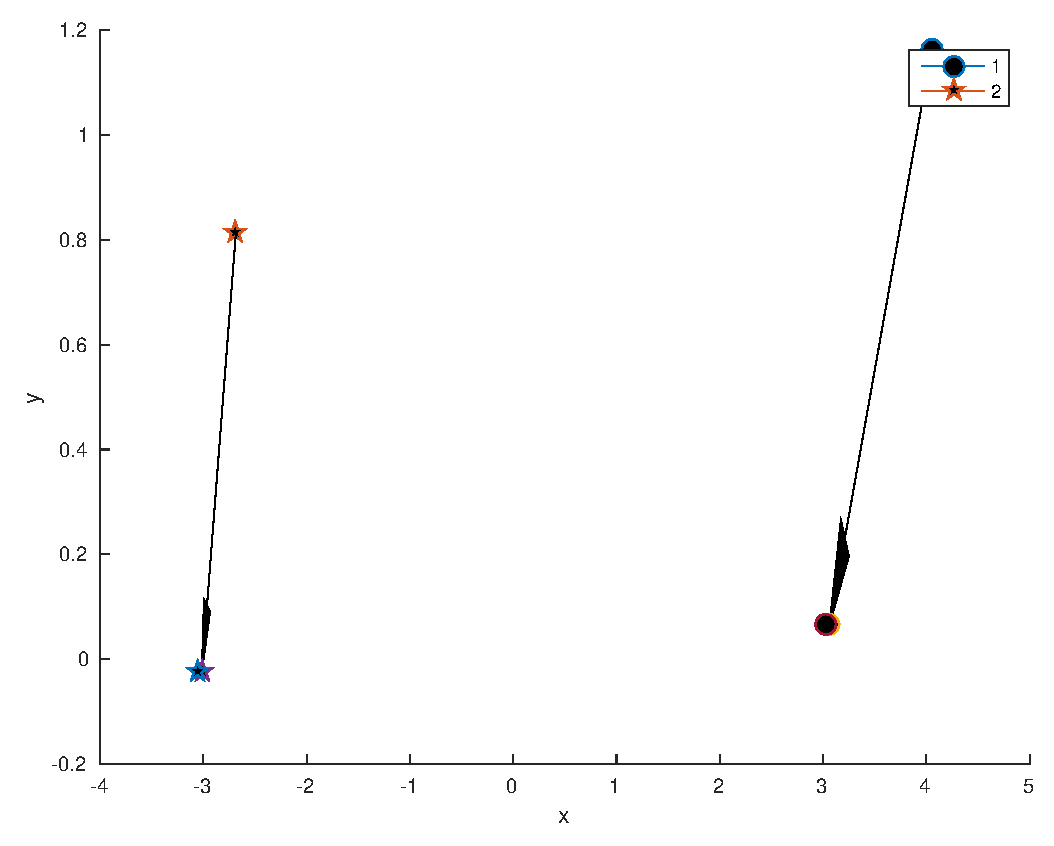
\includegraphics[width=\columnwidth]{Fig1_k2.eps}
    \caption{intermediate positions of the cluster means, 
    with their progress indicated by the arrows.}
  \end{subfigure}
  \quad
  \begin{subfigure}[b]{.45\textwidth}
    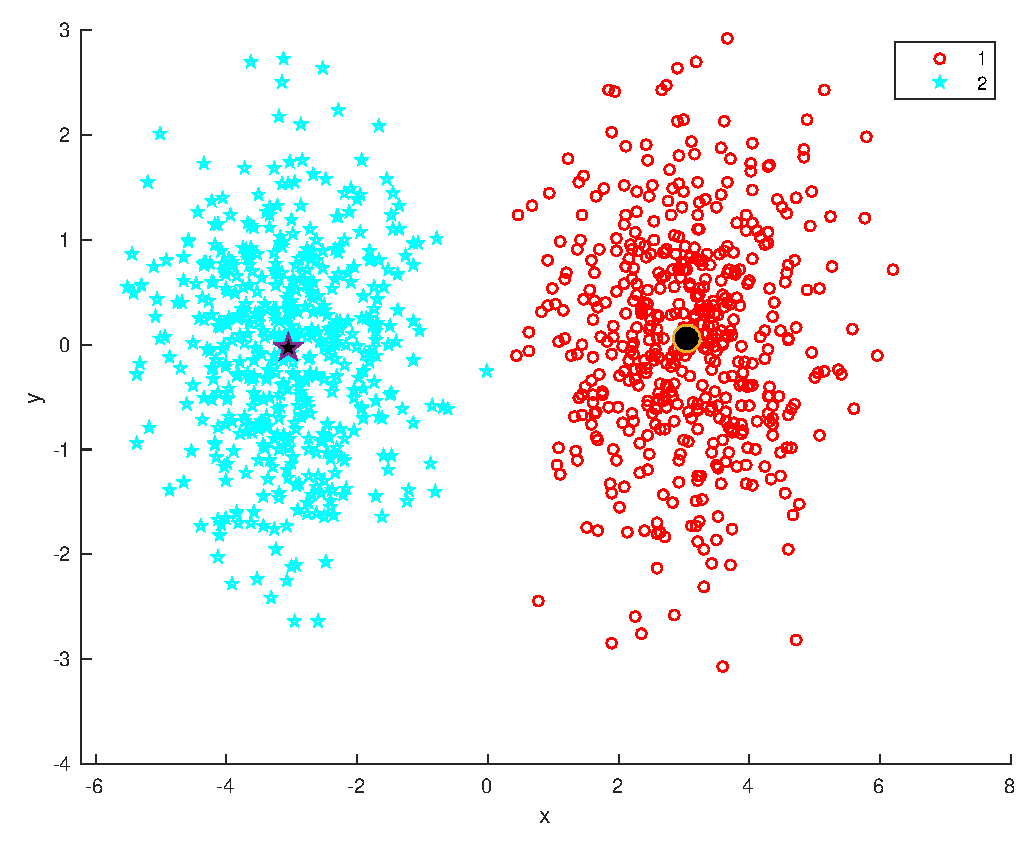
\includegraphics[width=\columnwidth]{Fig2_k2.eps}
    \caption{The final cluster means with their assigned data points)}
  \end{subfigure}
\end{figure}

\begin{figure}[H]
  \centering
  \caption{Results for k=4}
  \begin{subfigure}[b]{.45\textwidth}
    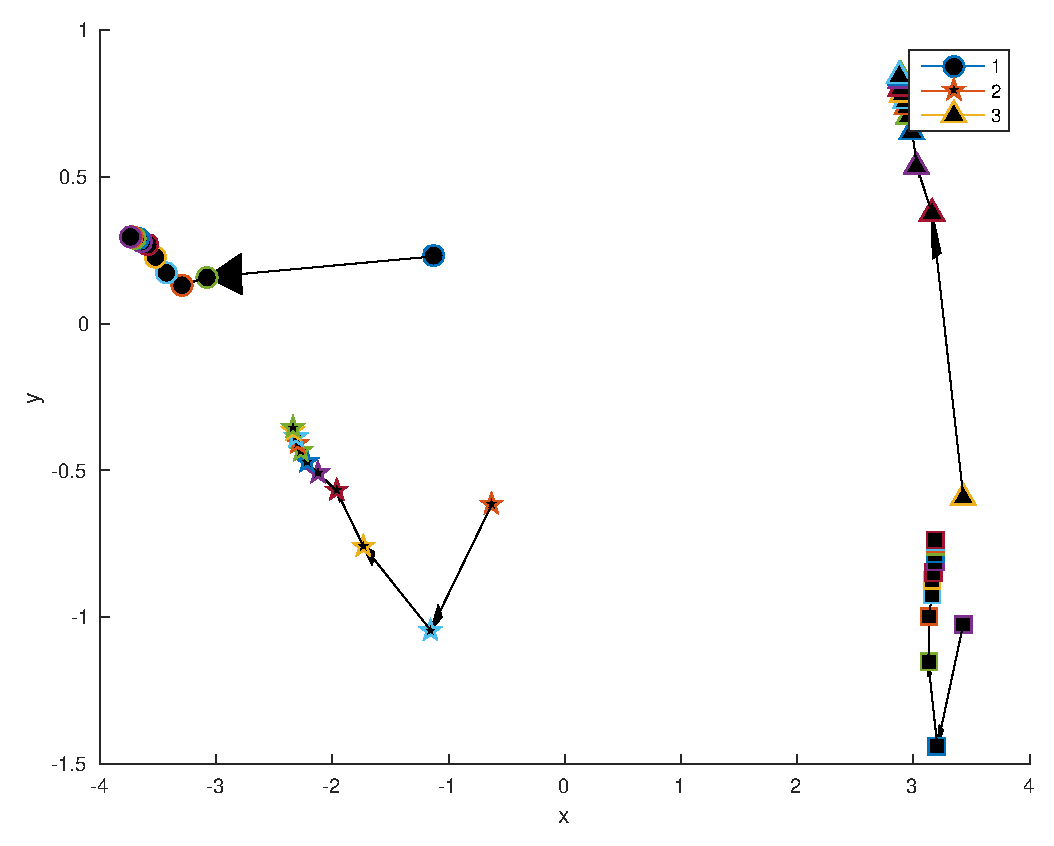
\includegraphics[width=\columnwidth]{Fig1_k4.eps}
    \caption{intermediate positions of the cluster means, 
    with their progress indicated by the arrows.}
  \end{subfigure}
  \quad
  \begin{subfigure}[b]{.45\textwidth}
    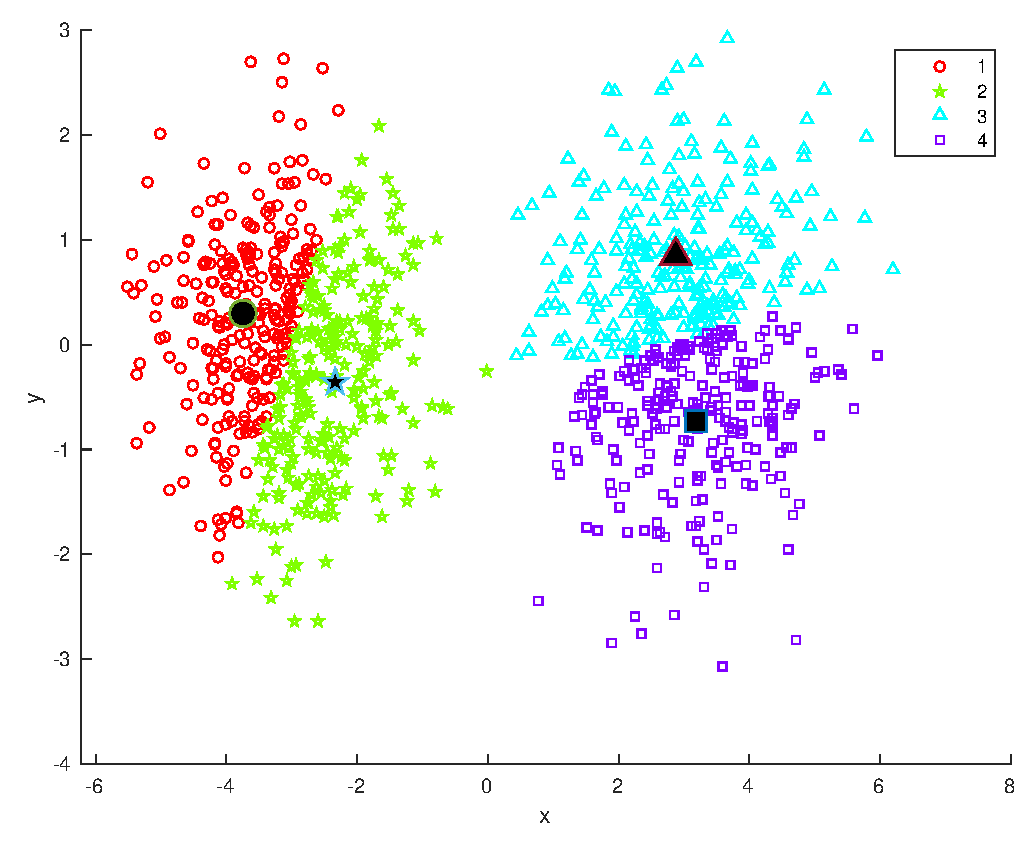
\includegraphics[width=\columnwidth]{Fig2_k4.eps}
    \caption{The final cluster means with their assigned data points)}
  \end{subfigure}
\end{figure}

\begin{figure}[H]
  \centering
  \caption{Results for k=8}
  \begin{subfigure}[b]{.45\textwidth}
    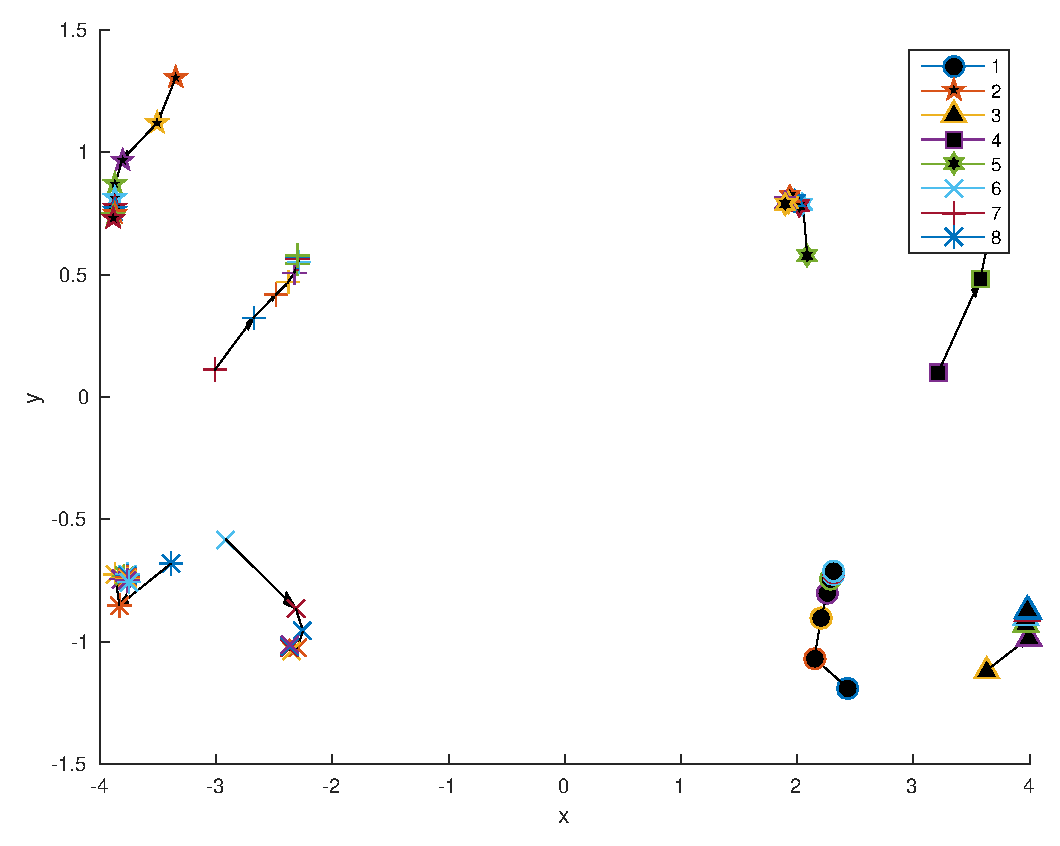
\includegraphics[width=\columnwidth]{Fig1_k8.eps}
    \caption{intermediate positions of the cluster means, 
    with their progress indicated by the arrows.}
  \end{subfigure}
  \quad
  \begin{subfigure}[b]{.45\textwidth}
    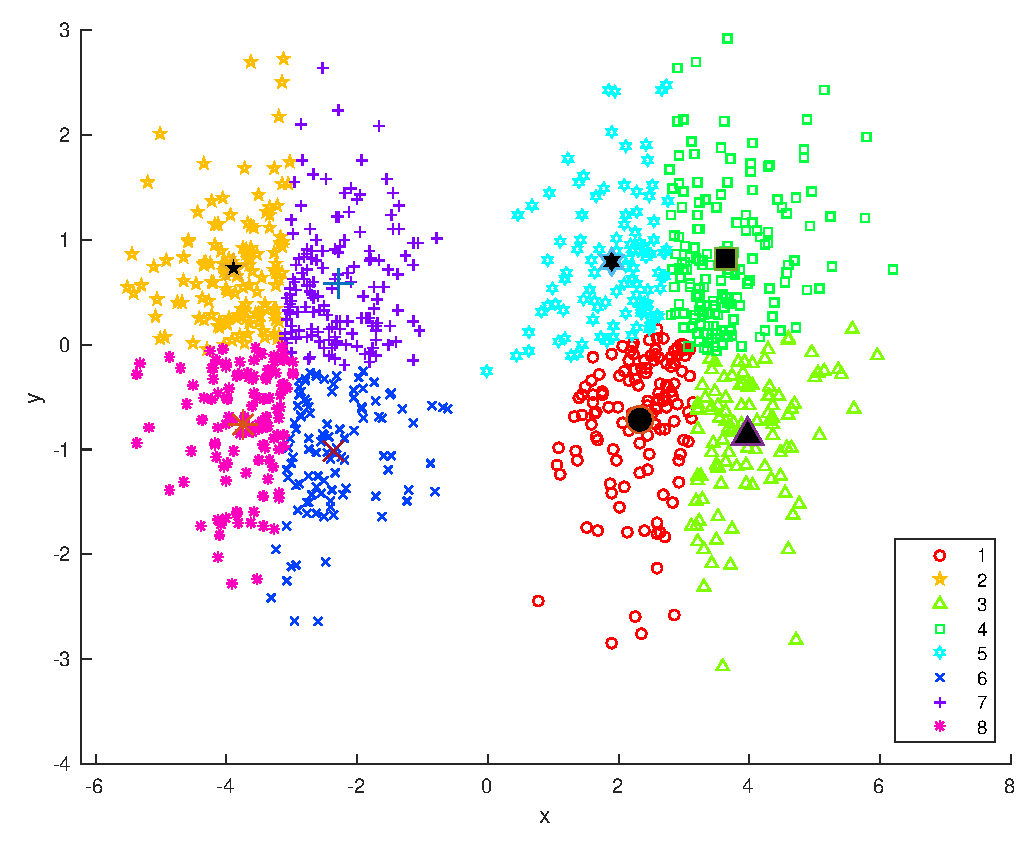
\includegraphics[width=\columnwidth]{Fig2_k8.eps}
    \caption{The final cluster means with their assigned data points)}
  \end{subfigure}
\end{figure}




\section{Batch Neural gas vs k-means}
\section*{Appendix}
\lstinputlisting{../Code/kmeans.m}{\label{kmeans}}
\lstinputlisting{../Code/runKMeans.m}{\label{runKMeans}}

\end{document}
